\chapter{Solutions of Non-Linear Equations}

\section{Bisection Method}

\thm{Intermediate Value Theorem}{
    If $f$ is continuous on $[a,b]$ and if $f(a)$ and $f(b)$ are non-zero and have opposite signs, then there is at least one solution of $f(x) = 0$ in the interval $(a,b)$ 
}

\begin{figure}[h]
    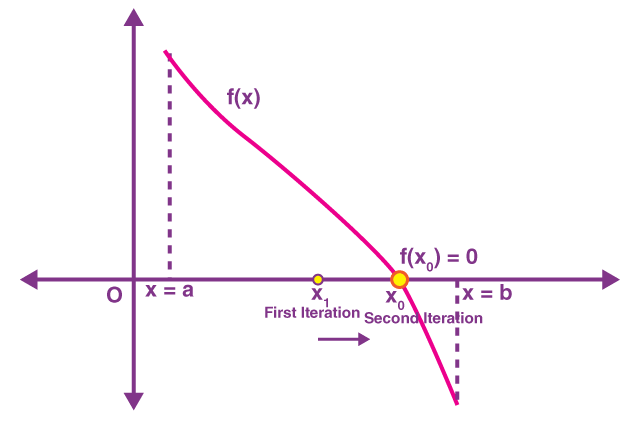
\includegraphics[width=12cm]{images/img-2-1.png}
    \centering
\end{figure}

\begin{algorithm}[H]
    For any continuous function $f(x)$, find a closed interval $[a, b]$ such that $f(a).f(b) < 0$. \\
    Find the midpoint of $a, b$. Let $x_1 = (a + b)/2$ \\
    \uIf{$f(x_1) = 0$}{
        then $x_1$ is the root. \\
    }
    \uIf{$f(x_1) \neq 0$}{
        \uIf{$f(a).f(x_1) < 0$}{
            Root of $f(x)$ lies in $[a, x_1]$, continue the above steps for interval $[a, x_1]$ \\
        }
        \Else{
            Root of $f(x)$ lies in $[x_1, b]$, continue the above steps for interval $[x_1, b]$. \\
        }
    }
    Continue the process repeatedly until we find a point $x_o$ in $[a, b]$ for which $f(x_o) = 0$. 
    
    \caption{Finding root of $f(x)$ using Bisection Method}
\end{algorithm} 

\thm{Error Analysis of Bisection Method}{
    If $f$ is a continuous function on $[a,b]$ and $f(a)\cdot f(b) < 0$ and let $\{c_n\}$ be a sequence generated using bisection method and let $c$ be the exact root of $f(x)=0$, then error at the $n^{th}$ interval is
    \begin{equation*}
        |c-c_n| \leq \frac{b-a}{2^n}
    \end{equation*}
}

\thm{}{
    The number of iterations $n$ required to obtain a approximating that is less than the tolerance $\epsilon$ is given by
    \begin{equation*}
        n \geq \frac{\log(b-a) - \log(\epsilon)}{\log(2)}
    \end{equation*}

    \begin{center}
        \begin{align*}
            n &\text{ is the number of iterations} \\
            a &\text{ is the lower bound of the interval} \\
            b &\text{ is the upper bound of the interval} \\
            \epsilon &\text{ is the tolerance} \\
        \end{align*}
    \end{center}
}